
\documentclass[11pt]{article}
\usepackage{natbib}
\usepackage{amssymb, amsmath}
\usepackage{common}
\usepackage{graphicx}
\graphicspath{ {../img/} }

\DeclareMathOperator{\E}{\mathbb{E}} % expected value
\newcommand{\bx}{\bm{x}}
\newcommand{\by}{\bm{y}}
\newcommand{\bz}{\bm{z}}
\newcommand{\Loss}{\mathcal{L}}

\title{HW4: Variational Autoencoders}
\author{Alex Lin \\ alexanderlin01@college.harvard.edu \and Melissa Yu \\ melissayu@college.harvard.edu}


\begin{document}

\maketitle{}
\section{Introduction}

\section{Problem Description}

\section{Model and Algorithms}

We explored the performance of a Variational Autoencoder and Generative Adversarial Network (and modifications of these models) on the MNIST digits dataset.

\subsubsection{Generative Adversarial Networks} \label{sssec:gan}
The generative adversarial network (GAN) (\cite{gan}) framework establishes a min-max game between two neural networks, the generator $G$ and the discriminator $D$, in order to match the generative process to the data distribution. Suppose the generator network $G(z)$ maps some latent representation $z\sim p(z)$ to the data space, and the discriminator network $D(x)$ predicts the probability that a sample $x$ comes from the true data distribution $p_d$ (positive samples), and not $G$'s generative process (negative samples). The objective is
\begin{equation}
\min_G \max_D \ \E_{p_d(x)} [\log D(x)] + \E_{p(z)} [\log (1 - D(G(z)))]
\end{equation}
The network consists of the discriminator, which achieves the best classification accuracy over samples of $x$, and the generator, which maximally confuses this best discriminator, so that $D(x) = 1/2$. The network is trained in two stages, by first updating the discriminator using both real and generated samples, and then updating the generator using noise samples.

\subsection{Variational Autoencoder}
\cite{vae}

\section{Experiments}


\subsection{Generative Adversarial Network} 
We normalize all images to have values between -1 and 1, and de-normalize the generated images for visualization purposes. Our final GAN model consists of a generator and discriminator. The discriminator comprises 2 linear layers with LeakyReLU activations, followed by a linear output layer with Sigmoid activation. The generator comprises 2 linear layers with LeakyReLU activations, followed by a linear output layer with Tanh activation. The hidden dimension size for both $D$ and $G$ is 256. Because the stability of the GAN game suffers when we have sparse gradients, we achieve better results using the LeakyReLU activation (with negative slope 0.2) instead of the ReLU activation.

We train $G$ to maximize $\log(D(G(z))$ instead of minimizing $\log(1-D(G(z)))$ (\cite{gan}). Note that the new form of the loss is functionally equivalent, but enables stronger gradients early in training when the discriminator can be very confident about samples from the generator. During training for GAN's, the discriminator can be trained for $k$ steps before updating the generator once; if the generator is trained ``too much'' without updating the discriminator, it may simply learn to map many values of $x$ to the same $z$ and fail to be expressive enough to capture the latent data distribution. We find that setting $k=1$ is sufficient for our purposes. For both the generator and discriminator, we use the Adam optimizer with learning rate 0.0005 and train the model for 300 epochs.

The input to the generator is a noise vector, which is sampled from a spherical normal prior $p(\mathbf{z}) = \mathcal{N}(\mathbf{0}, \mathbf{I})$.

Because the MNIST dataset also provided labels for the data, we additionally tried improving the model's generator by training the discriminator to also classify the samples. To do this, we implemented an auxillary GAN, which shared the first 2 layers of the generator's neural network, but whose output layer consisted of a linear layer and softmax activation. The results for this modified model appear similar to the original network, and are also shown below.

\begin{figure}[H]
	\begin{center}
		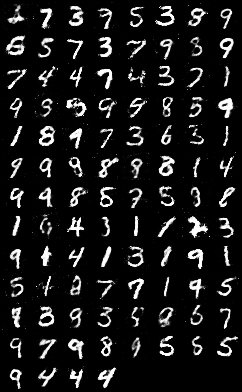
\includegraphics[scale=0.5]{fake_images-200}
		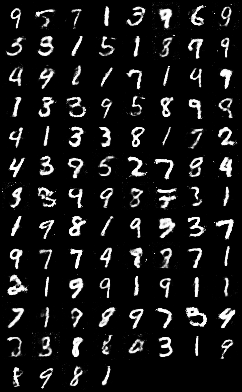
\includegraphics[scale=0.5]{fake_images-200-mod}
		\label{fig:gan-vis}
		\caption{Left: Visualization of 100 generated samples from random noise vectors sampled from a spherical normal prior with dimension 64. Right: 100 samples generated using the modified GAN with auxillary digit classification network.}
	\end{center} 
\end{figure}

\begin{figure}[H]
	\begin{center}
		
\includegraphics[scale=0.5]{interp_fake_images-1}
		
\includegraphics[scale=0.5]{interp_fake_images-2} \\
		
\includegraphics[scale=0.5]{interp_fake_images-1-mod}
		
\includegraphics[scale=0.5]{interp_fake_images-2-mod}
		\label{fig:gan-vis}
		\caption{Top: Visualization of samples generated from interpolations of 2 random noise vectors sampled from a spherical normal prior with dimension 64. Bottom: Interpolated samples generated using GAN with auxiliary network.}
	\end{center} 
\end{figure}

\subsection{Variational Autoencoder} 

\section{Conclusion}
In this practical, we implemented two models to generate written digit images: A Generative Adverasarial Network and a Variational Autoencoder.


\bibliography{writeup}
\nocite{*}
\bibliographystyle{apalike}

\end{document}
